\documentclass[dvipdfmx,autodetect-engine, 12pt]{jsarticle}

\usepackage{ulem} % 取消線を引くためのパッケージ
\usepackage[dvipdfmx]{graphicx} % 画像を挿入するためのパッケージ
\usepackage{array} % 表の幅指定や自動改行に必要
\usepackage{enumitem}

% --- 考文献用の設定 ---
\usepackage[backend=biber, style=numeric]{biblatex} % biblatexパッケージの使用
\addbibresource{report5.bib} % 先ほど作った別ファイルを指定（拡張子まで書く）
\usepackage{url} % WebサイトのURLを綺麗に出力するため

% --- section の文字サイズを小さくする設定 ---
\makeatletter
\renewcommand{\section}{%
  \@startsection{section}{1}{\z@}%
  {1.5ex \@plus .5ex \@minus .2ex}% 前の行との隙間
  {0.5ex \@plus .3ex}% 下の行との隙間
  {\normalfont\normalsize}% ← ここでサイズを \Large（少し大きめ）に指定
}
\makeatother

\begin{document}

% 課題のタイトル
\begin{center}

{\LARGE \bfseries 課題⑤\, iptablesによるポート転送\par}

\end{center}

\vspace{1cm}

{\LARGE \uline{目的}} \\

\hangindent=1.5zw
\hangafter=0
\noindent
iptables を用いたパケットの制御の実習を行う. パケットを分析することによりポート
転送の方法を確認する．

\vspace{1cm}

{\LARGE \uline{事前準備}} 

\begin{enumerate}
    \item server と router の VM を起動する．
    \item iptables コマンドについて調査する.
\end{enumerate}

\vspace{1cm}

{\LARGE \uline{手順}} 

\begin{enumerate}
    
    \item 2 台の VM（router と server）およびデスクトップ PC(Windows) を起動する．

    \item router で dropbear が起動していないことを確認し，起動している場合は停止する．
    
    \quad
    図\ref{fig:no_dropbear} は router で dropbear が起動していないことを確認する様子である．
    ps コマンドで プロセス一覧を取得し, その結果をgrep コマンドでdropbearという文字列を含むものに限定している.
    フィルタリングされたプロセス一覧には, grep dropbear(プロセス検索に用いたコマンド)以外のコマンドによるプロセスは表示されていない.
    したがって, routerにおいてdropbearが起動していないことが確認できる.

    \begin{figure}[htbp]
        \centering
        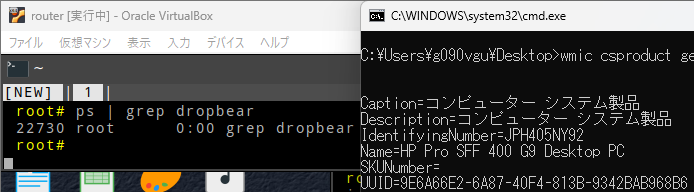
\includegraphics[width=0.8\textwidth]{imgs/no_dropbear.png} 
        \caption{server で dropbear が起動していないことを確認する様子}
        \label{fig:no_dropbear}
    \end{figure}

    \item server で dropbear を -R オプション付きで起動し，起動を確認する．
    
    \quad
    図は server で dropbear を -R オプション付きで起動し，起動を確認する様子である.
    ここではプロセス一覧において dropbear -R というコマンドで起動されたプロセスが表示されていることから, dropbearが-Rオプション付きで起動していることが確認できる.

    \item デスクトップ PC(Windows) から router へ ssh で一般権限ユーザでログインできないことを確認する．
    
    \quad
    図\ref{fig:ssh_failed} はデスクトップPCからrouterへのssh接続に失敗する様子である.
    ssh: connect to host 10.6.158.90 port 22: Connection refused というエラーメッセージが表示されており,
    \begin{figure}[htbp]
        \centering
        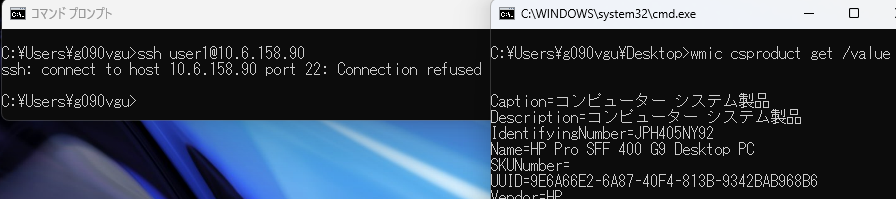
\includegraphics[width=0.8\textwidth]{imgs/ssh_failed.png} 
        \caption{デスクトップPCからrouterへのssh接続に失敗する様子}
        \label{fig:ssh_failed}
    \end{figure}

    \item router の組織外側インターフェースに対して以下の iptables 設定を行う（必要なら sysctl で転送を有効化：net.ipv4.ip\_forward=1）：
    
    \begin{enumerate}[label=\textcircled{\scriptsize\arabic*}]
        \item TCP 22 番ポート宛てのパケットを server の TCP 22 番ポートへ転送する（例：PREROUTING で DNAT を設定）。
        \item TCP のそれ以外のポート宛てアクセスは転送しない（DROP/REJECT を設定）。
    \end{enumerate}


    
    \item Windows から router へ通信を発生させ，server に一般権限ユーザでログインできることを確認する（必要に応じて known\_hosts を編集して Host key 問題を解決する）．
    
    \quad
    図\ref{fig:ssh_login_success} はデスクトップPCからrouterへのssh接続を試みた結果である.
    先程は失敗したssh接続が成功していることがわかる.

    \begin{figure}[htbp]
        \centering
        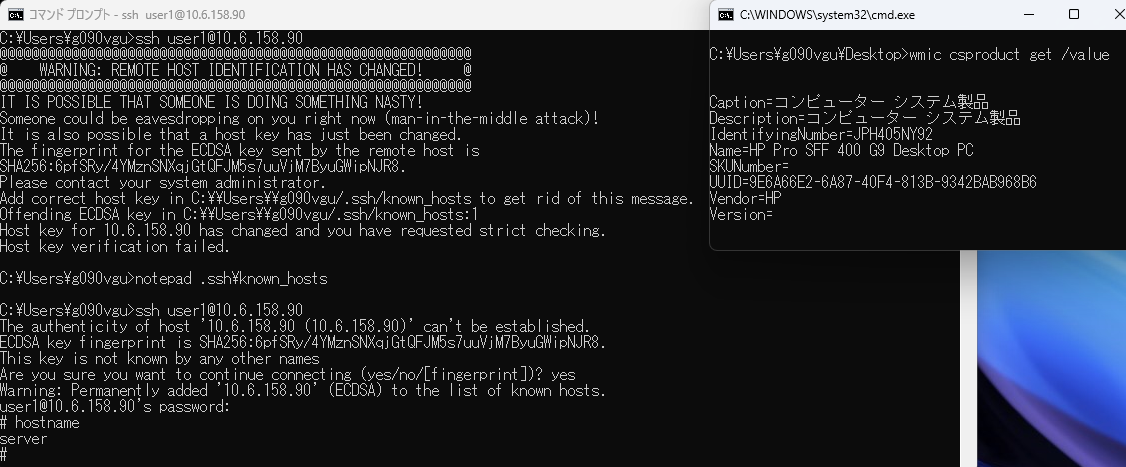
\includegraphics[width=0.8\textwidth]{imgs/ssh_win2sever_via_router.png} 
        \caption{デスクトップPCからrouterへのssh接続に成功する様子}
        \label{fig:ssh_login_success}
    \end{figure}

    \item router 上で Wireshark を起動し，Windows↔router および router↔server の両方のインターフェースをキャプチャ対象に設定する．

    \item Windows から router への SSH ログイン過程のパケットを router の Wireshark で解析し，iptables による転送（IP アドレスやポート番号の書き換え）が観測できるパケットを特定する．
    
    \quad
    図\ref{fig:ssh_login_result}はrouter上でWiresharkを起動し, Windows↔router および router↔server の両方のインターフェースをキャプチャ対象に設定した様子である.
    ここではキャプチャするパケットは, Windows↔router および router↔server を流れるパケットにに限定するため, wiresharkのフィルタに
    (ip.src==192.168.100.1 and ip.dst==192.168.100.2) or (ip.src==192.168.100.2 and ip.dst==192.168.100.1)
    と
    (ip.src==10.6.158.90 and ip.dst==10.6.158.153) or (ip.src==10.6.158.153 and ip.dst==10.6.158.90)
    を設定している.
    前述のようにフィルタリングした上で, 両方のインターフェースを流れるパケットを比較すると, プロトコルやパケット内の情報が酷似していることが確認できる.
    実際に, １つパケットを抽出して比較した例を図\ref{fig:same_packet_example}に示す.
    TCPより上位の層において, すべてのフィールドの値が完全一致していることがわかる.

    \begin{figure}[htbp]
        \centering
        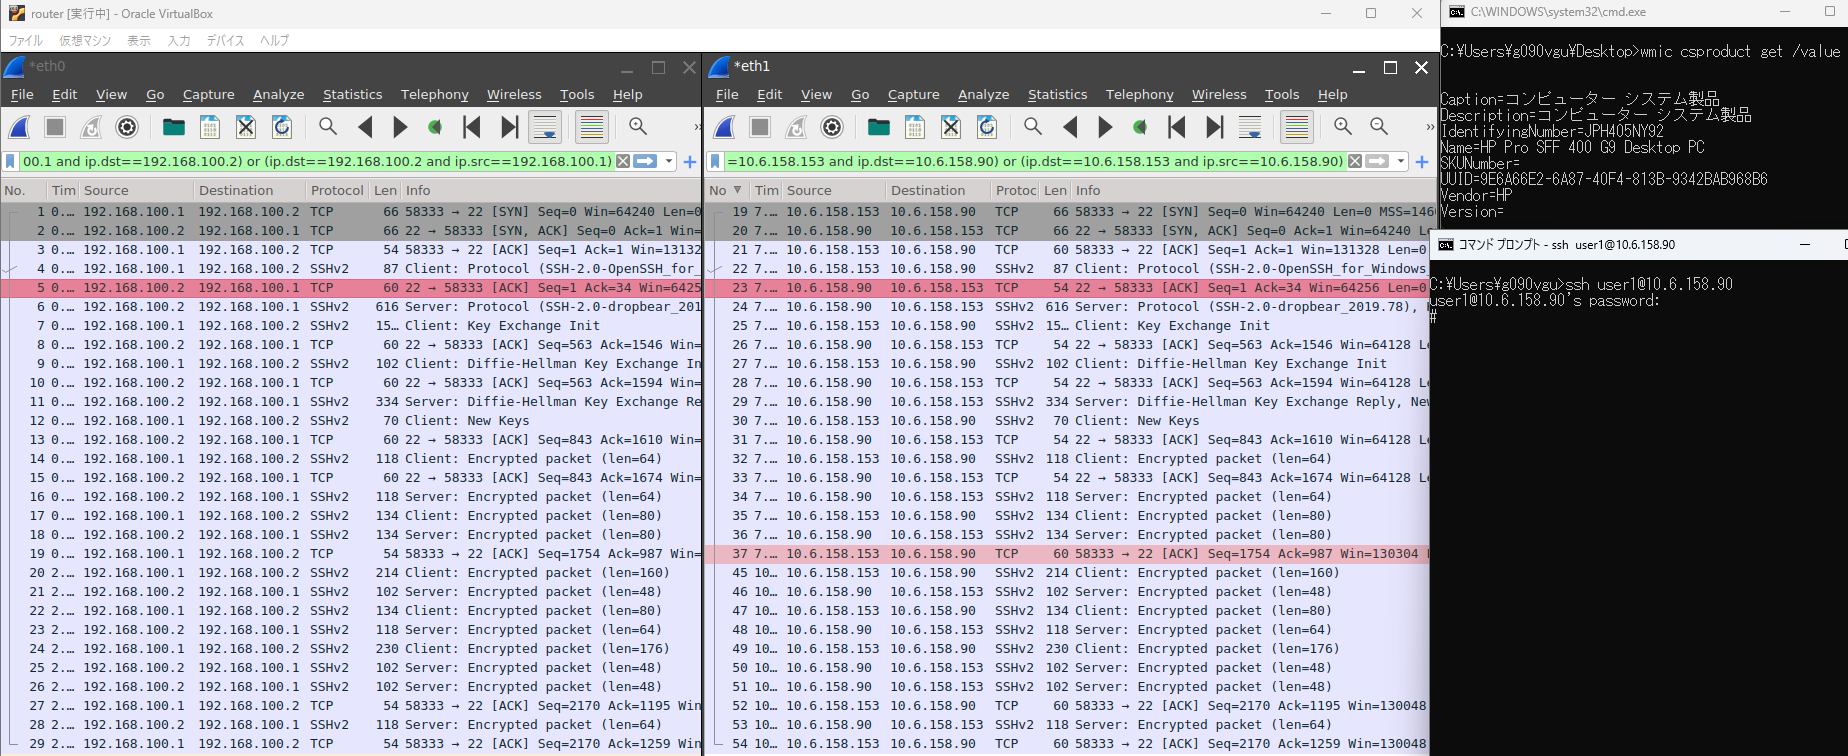
\includegraphics[width=0.8\textwidth]{imgs/ssh_login_result.png} 
        \caption{sshログイン時のWiresharkのキャプチャ結果}
        \label{fig:ssh_login_result}
    \end{figure}

    \begin{figure}[htbp]
        \centering
        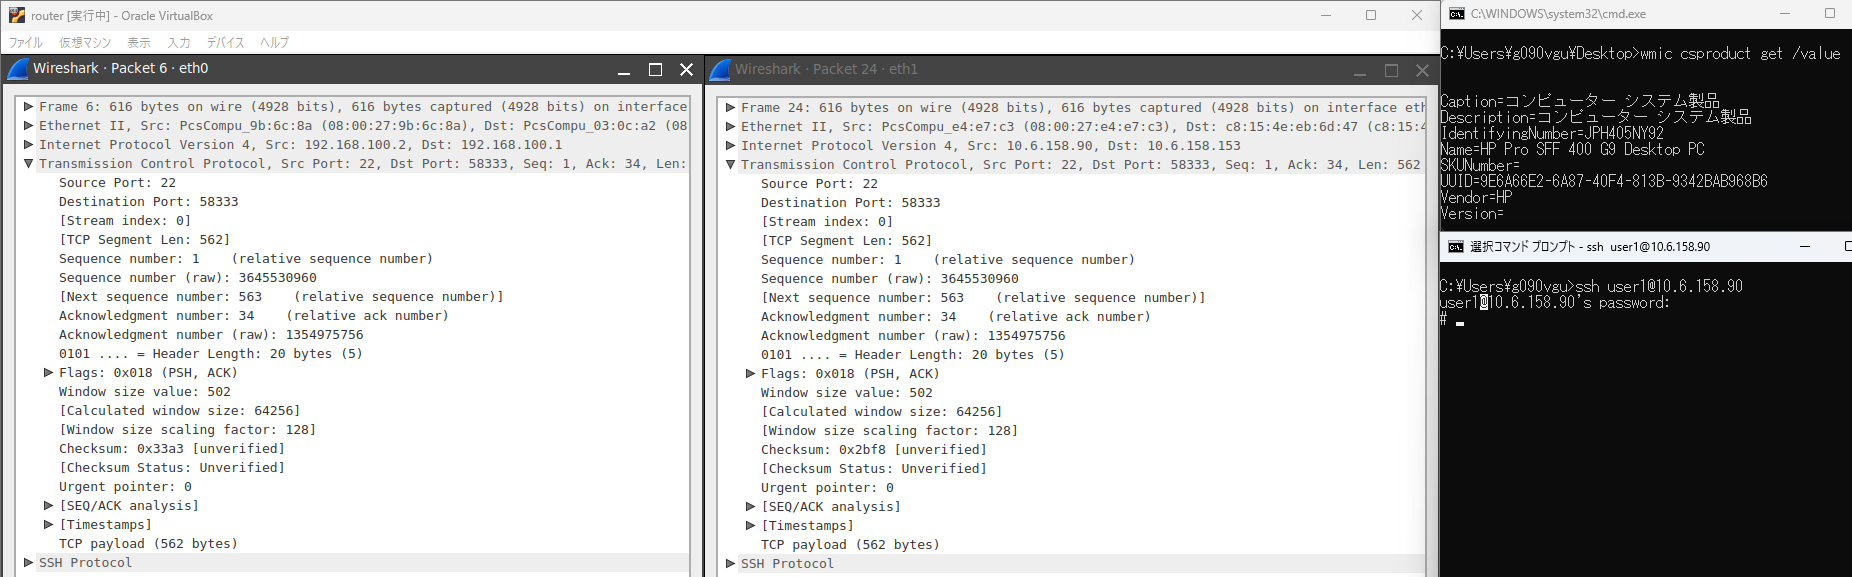
\includegraphics[width=0.8\textwidth]{imgs/same_packet_example.png} 
        \caption{Windows↔router および router↔server を流れるパケットの比較例}
        \label{fig:same_packet_example}
    \end{figure}
    
    \item router の組織内側インターフェースに対して，server から組織外側ネットワークへの通信が可能になるように iptables を設定する（例：POSTROUTING で SNAT/MASQUERADE を設定）．
    
    \item server から組織外ネットワークの端末へ通信を発生させ，router の Wireshark で解析し，iptables による変換（送信元 IP の書き換え等）を示すパケットを特定する．
    
    \item 実験結果として，デスクトップ PC から server へログインできること，server から組織外ネットワークへ通信できることを示し，使用したすべての iptables 設定を列挙する．各設定がどのようにパケットを書き換え，転送処理を実現しているかを具体的に説明してレポートにまとめる．

\end{enumerate}

\newpage

% --- 参考文献リストの出力 ---
\printbibliography[title=参考文献]

\end{document}